\newpage 

\section{Trigonometry Checkup}
These notes are intended to provide reminders of key ideas from high school trigonometry. 

\subsection{Right Triangle Trigonometry}
\begin{prob}
What are the ratios of side lengths in a $45^\circ$-$45^\circ$-$90^\circ$ triangle?  Explain where the ratios come from, including why they work for any triangle, no matter what size.  (Hint: Use the Pythagorean Theorem.)
\end{prob}

\begin{prob}
What are the ratios of side lengths in a $30^\circ$-$60^\circ$-$90^\circ$ triangle?  Explain where those the come from.  (Hint: Think of half of an equilateral triangle.)
\end{prob}

\begin{prob}
Consider the right triangle below with an angle of $\alpha$, sides of length $x$ and $y$, and hypotenuse of length $r$, as labeled.  
$$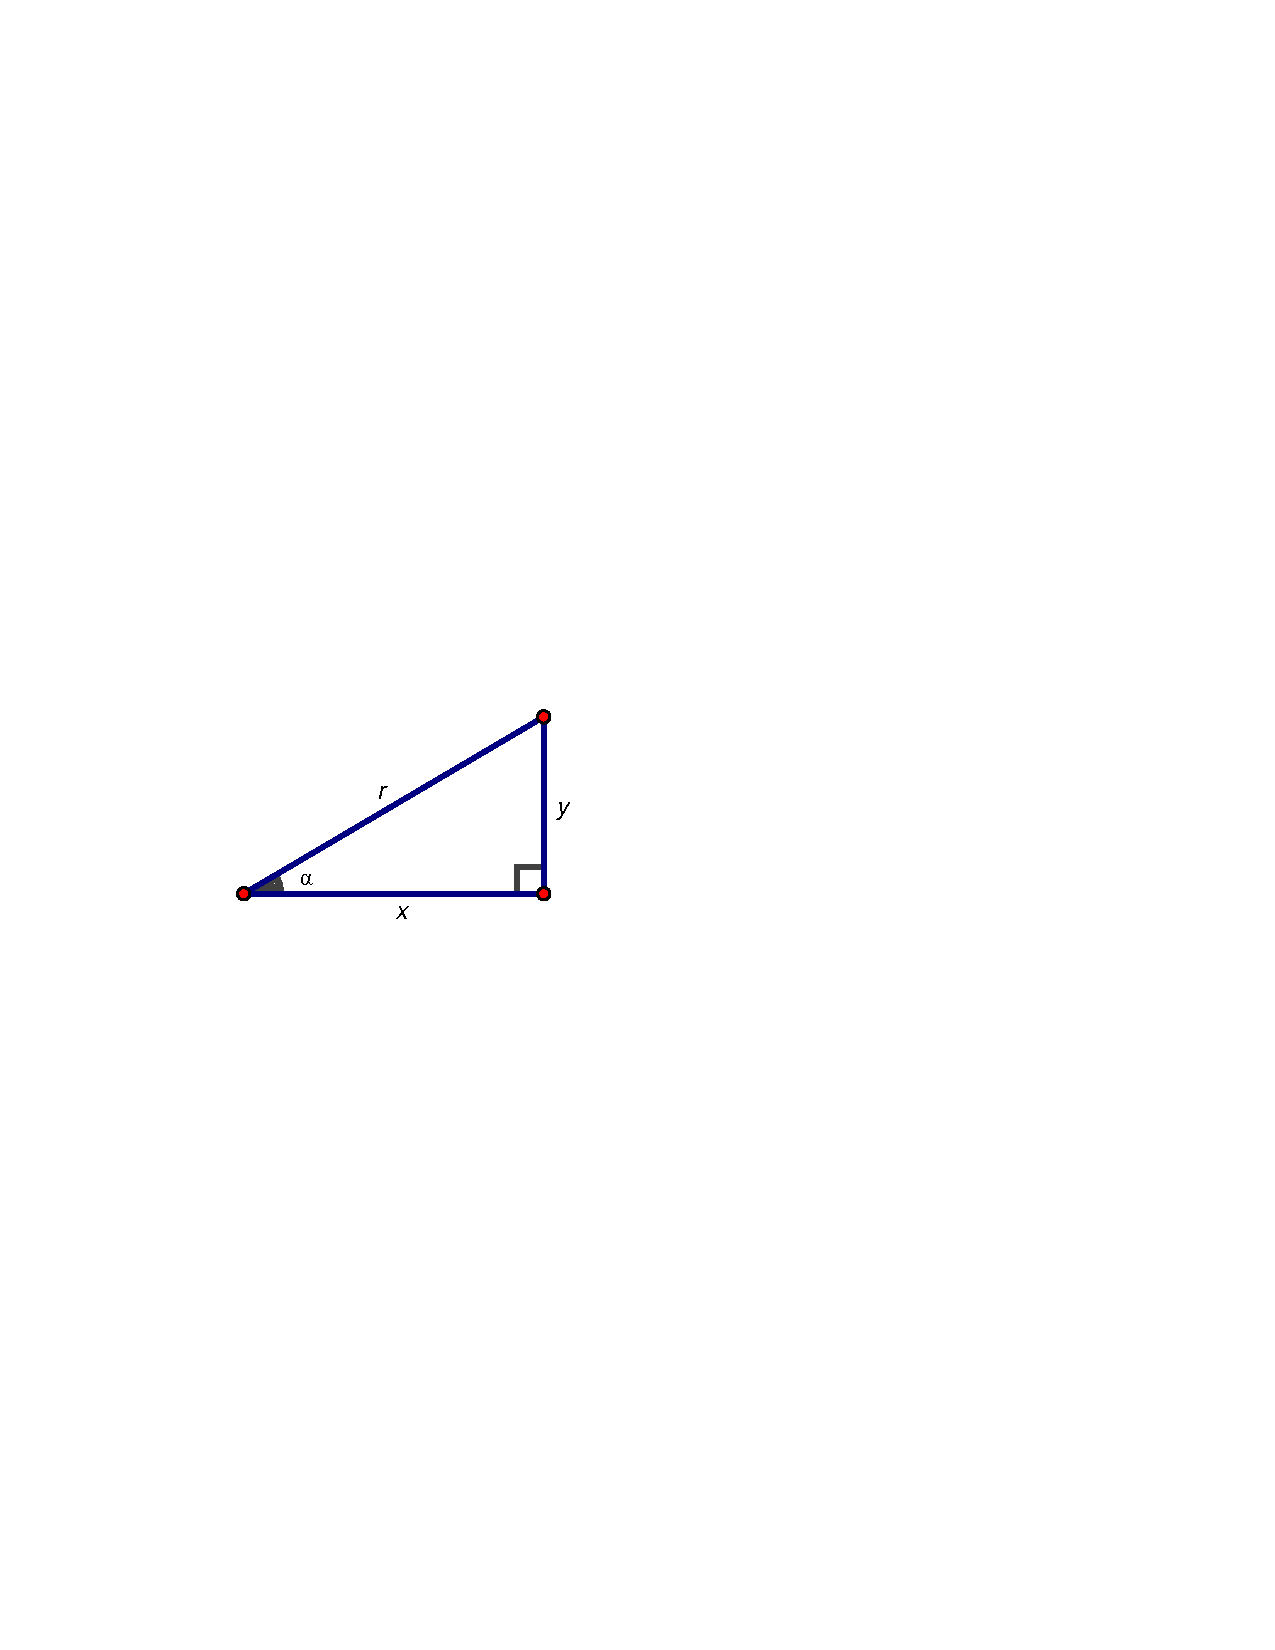
\includegraphics[scale=0.8]{../graphics/rightTriangle}$$
\begin{enumerate}
\item If we imagine angle $\alpha$ is fixed, why are ratios of pairs of side lengths the same, no matter the size of the triangle?\standardhs{G-SRT.6}
\item Using the triangle above (and your memory of Precalculus), write down the side-length ratios for sine, cosine, and tangent:  
$$\sin\alpha = \hspace{1in} \cos\alpha = \hspace{1in} \tan\alpha =$$
\item What does it mean to say that these ratios depend upon the angle $\alpha$?  
\item Why is only one angle necessary in defining these ratios?  
\item The discussion so far is about \emph{right triangle trigonometry}, in which the specified angle is always acute.  Explain why this limitation makes sense at this point.  
\end{enumerate}
\end{prob}

\begin{prob}
Use your work so far to find the following trigonometric ratios:
\begin{enumerate}
\item $\sin 30^\circ = \hspace{1in} \cos30^\circ = \hspace{1in} \tan30^\circ =$
\item $\sin 45^\circ = \hspace{1in} \cos45^\circ = \hspace{1in} \tan45^\circ =$
\item $\sin 60^\circ = \hspace{1in} \cos60^\circ = \hspace{1in} \tan60^\circ =$
\item $\sin 0^\circ = \hspace{1.08in} \cos0^\circ = \hspace{1.08in} \tan0^\circ =$
\end{enumerate}
\end{prob}

\begin{prob}
You may recall the identity $\sin^2\theta+\cos^2\theta=1$.\standardhs{F-TF.8}  
\begin{enumerate}
\item Explain why the equation is true.  
\item Why is it called an identity? 
\item Why is it called a Pythagorean identity?  
\end{enumerate}
\end{prob}

\begin{prob}
In right triangle trigonometry, there are indeed two acute angles, as shown in the figure below.\standardhs{G-SRT.7}
$$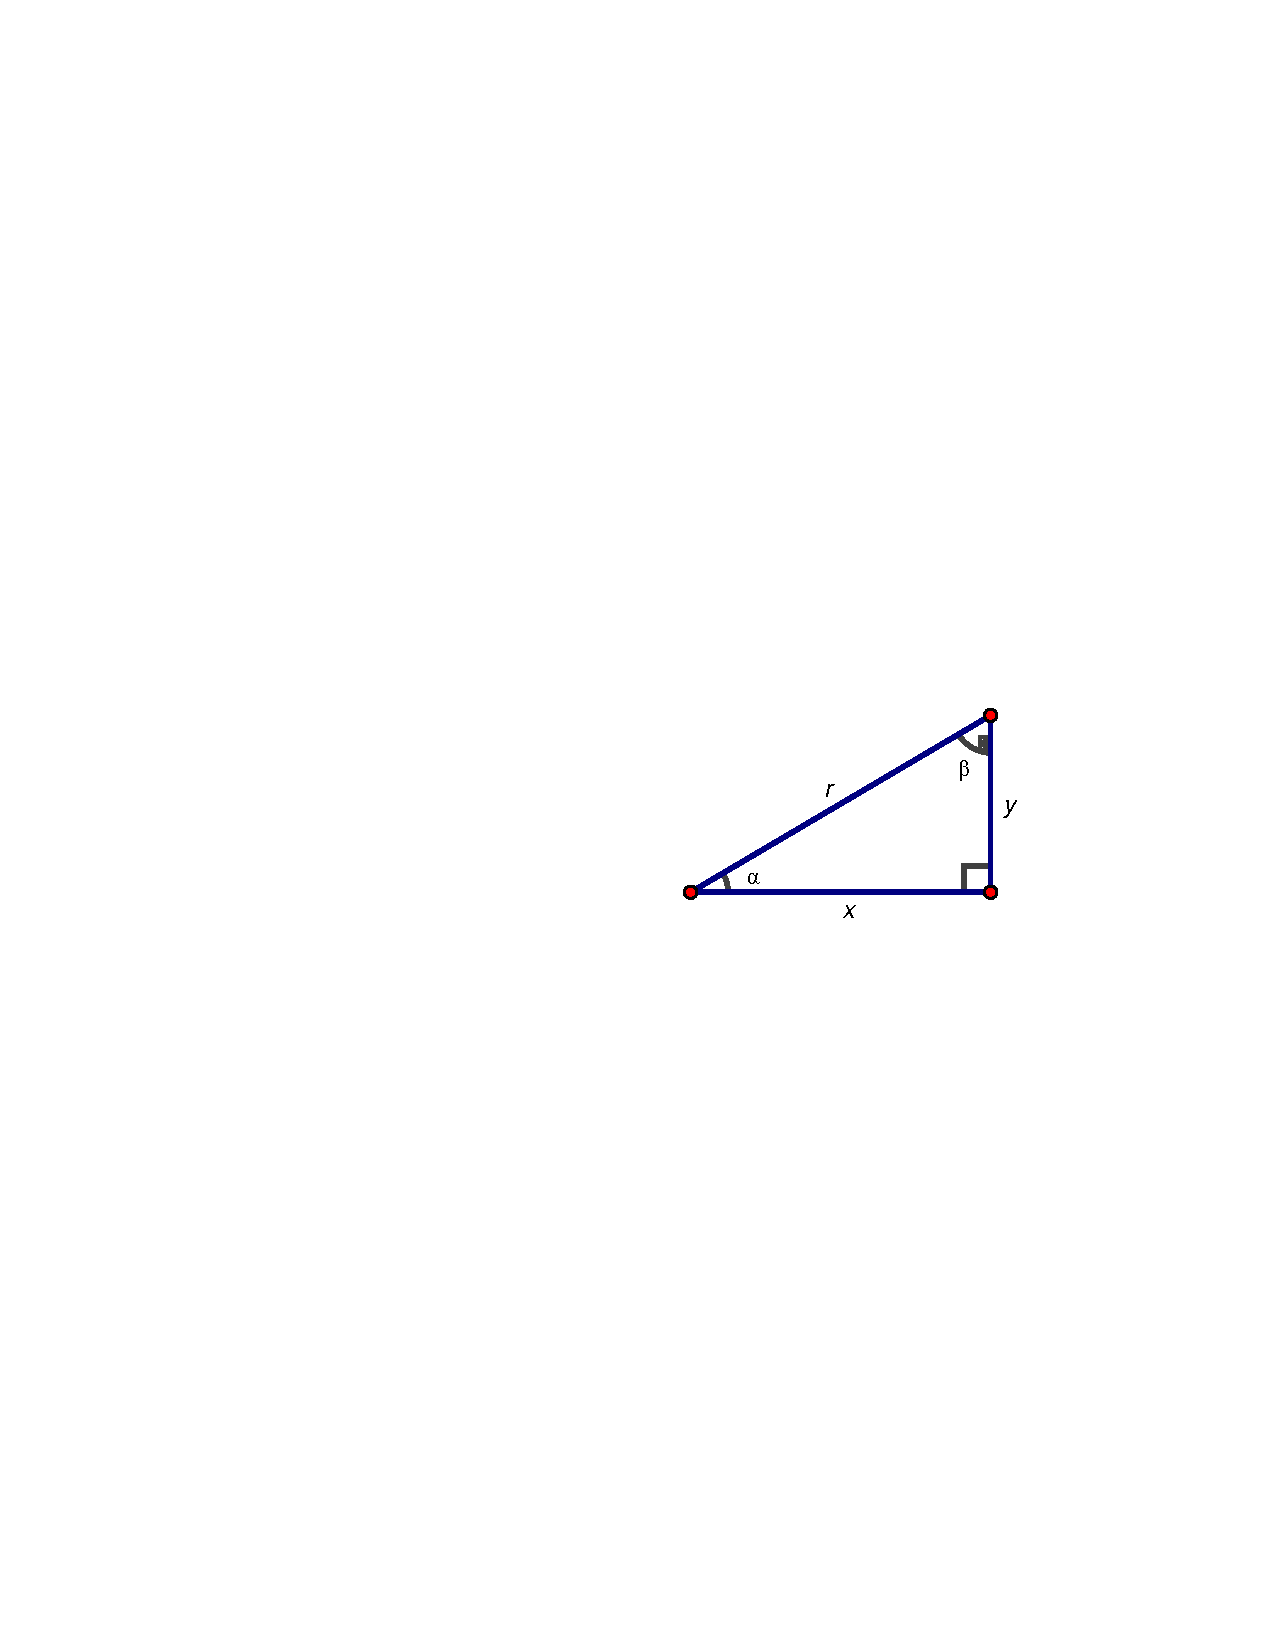
\includegraphics[scale=0.8]{../graphics/rightTriangle2}$$
\begin{enumerate}
\item How are the angles $\alpha$ and $\beta$ related?  Explain why.
\item Using lengths in the above triangle, find the following ratios:    
$$\sin\alpha = \qquad\qquad \cos\alpha = $$
$$\sin\beta = \qquad\qquad \cos\beta = $$
\item What do you notice about the sine and cosine of complementary angles?  
\item Explain why the result makes sense.  
\end{enumerate}
\end{prob}

Given an angle and a side length of a right triangle, you can find the missing side lengths.\standardhs{G-SRT.8}  This is called ``solving the right triangle.''  (Hint: Draw the triangle.)  \fixnote{The standard G-SRT.8 seems to have disappeared.}

\begin{prob}
A straight wire to the top of a flagpole meets the ground at a $25^\circ$ angle 30 feet from the base of the flag pole (on a flat lawn).  How high is the flagpole?  How long is the wire?  
\end{prob}

Given the sine, cosine, or tangent of an angle, you can find the other two ratios.  (Hint: Draw a triangle.)

\begin{prob}
Suppose $\sin\alpha = \frac{3}{5}$.  Then $\cos\alpha = \hspace{0.6in}$, $\tan\alpha = \hspace{0.6in}$.  
\end{prob}

\subsection{Circular Trigonometry}
As we have seen, right triangle trigonometry is restricted to acute angles.  But angles are often obtuse, so it is quite useful to extend trigonometry to angles greater than $90^\circ$.  Here is one approach:  Place the angle with the vertex at the origin in the coordinate and with one side of the angle (the initial side) along the positive $x$-axis.  Measure to the other side of the angle (the terminal side) as a counter-clockwise rotation about the origin.   

%\begin{prob}
%Now we can find the area of a triangle given two sides and an angle.\standardhs{G-SRT.9}  
%\end{prob}
%
%% Laws of Sines and Cosines \standardhs{G-SRT.10}, \standardhs{G-SRT.11}

Because angles are often about rotation, angles greater than $180^\circ$ can make sense, too.  And negative angles can describe rotation in the opposite direction.  If we consider the angle to change continuously, then rotation about the origin creates a situation that repeats every $360^\circ$.  This repetition provides the foundation for modeling lots of repetitive (periodic) contexts in the real world.  For this modeling, we need \emph{circular trigonometry}, which turns out to be much cleaner if (1) angles are measured not in degrees but in a more ``natural'' unit, called radians; and (2) we use \emph{the unit circle}, which is a circle of radius 1 centered at the origin.   The steps are as follows:  

\begin{enumerate}
\item Understanding radian measure.\standardhs{G-C.5}, \standardhs{F-TF.1}

\item Using the unit circle to extend trigonometry to angles of any measure.\standardhs{F-TF.2}

\item Choosing and using trig functions to model periodic phenomena.\standardhs{F-TF.5}

\end{enumerate}

\fixnote{Complete this section.}
% Fluency finding trig functions of special angles in radian measure.\standardhs{F-TF.3}

